\documentclass[sigconf, anonymous=false, screen=true]{acmart}

%% HotMobile 2027 submission — 8-page version with all 7 review patches applied.
%% Source: user's HotMobile draft + 7 patches (Challenges, prior-art gap,
%% Goals, n=7 fix, LongBench K=512, closed-loop framing, reproducibility).

\settopmatter{printacmref=false}
\renewcommand\footnotetextcopyrightpermission[1]{}
\pagestyle{plain}

\usepackage{booktabs}
\usepackage{tabularx}
\usepackage{multirow}
% compact yes/no marks for the related-work table (tab_related_mobile.tex)
\newcommand{\yes}{$\bullet$}
\newcommand{\no}{--}

\usepackage{xcolor}
\usepackage{hyperref}
\usepackage{microtype}
\usepackage{graphicx}
\graphicspath{{figures/}}
\usepackage{algorithm}
\usepackage{algpseudocode}
\usepackage{enumitem}

%% --- Column-overflow control (added 2026-07-26) ---------------------------
%% TeX cannot break a text-mode "/" or an inline \mathrm{clip}(...) group, and
%% cannot hyphenate \texttt identifiers, so slash-ladders, long code names and
%% wide inline math were bleeding up to 118pt past the column edge.
%% \slb = breakable slash; \ub = breakable underscore; emergencystretch soaks
%% up the remaining small (<25pt) text overflows.
\newcommand{\slb}{/\allowbreak}
\newcommand{\ub}{\_\allowbreak}
\setlength{\emergencystretch}{2em}

\definecolor{kvgreen}{RGB}{40, 174, 96}
\definecolor{kvred}{RGB}{192, 57, 43}
\definecolor{kvgray}{RGB}{85, 85, 85}
\newcommand{\good}[1]{\textcolor{kvgreen}{\textbf{#1}}}
\newcommand{\bad}[1]{\textcolor{kvred}{\textbf{#1}}}
\newcommand{\nodata}{\textcolor{kvgray}{\textit{---}}}
\newcommand{\circled}[1]{\raisebox{.5pt}{\textcircled{\raisebox{-.9pt}{\footnotesize #1}}}}

\begin{document}

%% Short running title (added 2026-07-26): the full title overflowed the running
%% head and collided with the venue string on every odd page.
%% TITLE CHANGED 2026-08-17 (same correction as the 2027 file, see its comment):
%% the old title claimed a loop that never closes at runtime, an actuator \S6 refutes,
%% and led with the per-head gate against the paper's own realizability finding.
\title[$\mu$KV: Energy- and Thermal-Aware KV Eviction on a Phone]{$\mu$KV: Energy- and Thermal-Aware KV-Cache Eviction for LLM Inference on a Phone}

\author{Md Romyull Islam}
\affiliation{%
  \institution{Kennesaw State University}
  \city{Marietta}
  \state{Georgia}
  \country{USA}
}
\email{romyullislam2012@gmail.com}

\begin{abstract}
%% ABSTRACT REPLACED 2026-08-17 with the corrected one (see PAPER_HOTMOBILE_2027.tex
%% for the change rationale): the old text carried 4.8x/62% from a single cold-start
%% cell, the handicapped StreamingLLM, and the retired round-trip mechanism.
On a phone the KV cache, not compute, limits sustained LLM decode. But the policies that bound it were designed for server GPUs, and three properties of a real on-device inference engine break them. \emph{(i)} The cell array is shared across heads and layers, so a cell is freed only if \emph{every} per-head selector dropped it; SnapKV's nominal per-head budget retains 67.7\% of cells on Llama-3.2-1B and 84.9\% on Phi-3-mini, and H2O's 20\%-of-context ratio retains 99.8\%. Their budgets never materialize on the device. \emph{(ii)} Reading post-softmax attention forces the FlashAttention-off path, which on device costs more than eviction saves: those policies decode at 0.10--0.19$\times$ the full cache across three backends. \emph{(iii)} Compacting through the engine's state API needs a second full context, exceeding unified memory --- Phi-3-mini at 16K is killed by the OS on the phone and fails identically on a 24\,GB desktop GPU. We present $\mu$KV, which respects all three: it computes selection scores \emph{inside} the FlashAttention prefill graph through a small side node, so it obtains the attention signal without leaving the fast path; it selects one sequence-level keep-set, so eviction actually frees cells; and it compacts \emph{in place}, sliding survivors into a dense prefix inside the tensors prefill already allocated, so peak memory never rises. On a OnePlus 15, $\mu$KV retains 7.4\% of cells and decodes 1.20$\times$ faster than the full cache while every per-head baseline is 0.10--0.19$\times$. A faithfully configured StreamingLLM --- its own 2004-cell budget, flash-attention on, and the contiguous keep-set its own implementation maintains --- also reaches 1.20$\times$, so keeping FlashAttention on, not evicting more, is what governs on-device speed; $\mu$KV's advantage over it is that it reaches the same throughput on 2.8$\times$ fewer cells and retrieves 14/14 needles against its 7/14. Under sustained load $\mu$KV finishes eight back-to-back 4096-token generations in 1.21$\times$ less wall time at 1.60$\times$ decode throughput, and in-place compaction makes Phi-3-mini at 16K feasible where the state round-trip is killed. At 64K, $\mu$KV retains 1.4\% of the cache at \emph{lower} perplexity than the full cache (10.42 vs 11.05) on a WikiText slice verified disjoint from the prompt. We report costs as plainly as wins: prefill is 1.06$\times$ slower (the scoring cost); peak resident set is \emph{higher} than vanilla's, because the KV buffer is allocated at full context up front, so the win is in retained cells and bandwidth, not footprint; a disjoint-slice perplexity shows eviction does not damage language modeling but cannot show that prompt information survives, which is what retrieval measures; and coupling cache size to temperature does not cap heat, so frequency remains the thermal lever and the cache an efficiency lever.
\end{abstract}

\keywords{Mobile LLM inference, KV cache eviction, FlashAttention, thermal management, energy efficiency, Snapdragon, on-device AI}

\maketitle

\section{Introduction}
\label{sec:intro}

\paragraph{Motivation.} Phone LLM workloads differ from a server's: a single user, a 30--60\,s sustained generation, a thermal envelope that throttles long before any compute limit, and an OS that kills the process past a memory-headroom threshold. Quality is necessary but not sufficient; a policy that wins perplexity at the cost of skin temperature, peak resident-set, or battery drain fails deployment. The literature optimizes \emph{one} axis at a time (perplexity, DVFS, or compression alone), but the phone couples all of them: cache size sets DRAM read, read sets power, power sets temperature, temperature sets throttle, throttle sets throughput. A mobile KV-cache policy must be jointly evaluated on \emph{quality} (NIAH, LongBench, perplexity), \emph{throughput} (decode tps at realistic 16K context), and \emph{thermal} (peak DDR vs the kernel cliff, peak skin, watchdog activity), on real hardware. The literature has nothing that does all three on a phone.

\paragraph{Problem.} Small instruction-tuned LLMs (1--4B parameters, 4-bit quantized) now run interactively on flagship phones at 5--7 tokens/s on CPU. The remaining wall is not the matrix multiply; it is the KV cache. Once sustained generation passes a thousand tokens, four pressures bind at once:

\begin{itemize}
\item \textbf{Cache size.} A Phi-3-mini cache at 2K holds about 1.2\,GiB (f16 K+V). On a 12\,GB phone shared with foreground apps this triggers swap: 158\,MB of swap-out under the full cache, swap-in stalls near 280\,ms.
\item \textbf{DRAM bandwidth.} Decode reads the whole cache once per layer per token, roughly 750\,MB per attention pass for Phi-3 at 2K. On LPDDR5X (${\sim}50$\,GB/s) this dominates the step.
\item \textbf{Thermals.} The Qualcomm BCL~\cite{qualcommbcl} and the kernel cooling driver cut the big-core clock from 1632 to 883\,MHz once DDR passes about 65\,\textdegree C, often within 90\,s of sustained decode.
\item \textbf{Energy.} A full-cache 2048-token decode draws about 38.7\,mAh; on a 5000\,mAh battery that is about 130 generations before any other app load.
\end{itemize}

\paragraph{Five design challenges.} A phone-viable evictor must resolve five tensions together. (i) Any per-head signal from post-softmax attention is locked out of FlashAttention, the kernel that makes mobile decode fast. (ii) q8\ub 0 K quantization only pays above roughly a 1\,GB cache. (iii) Aggressive eviction runs \emph{hotter} at peak, not cooler, because freed bandwidth converts to clock and power. (iv) A fixed $K$ wastes headroom on short prompts while a fraction-of-prompt $K$ blows the DRAM budget on long ones. (v) At a tight budget the same ramp tunes either for chat throughput or document-QA quality, so the split should be chosen per request from a cheap prefill signal.

These pressures are coupled, and one intervention --- bounding the cache by a per-head confidence-aware budget --- pushes on all four at once.

The policies that could supply that bound were designed elsewhere: H2O~\cite{zhang2023h2o}, TOVA~\cite{oren2024tova}, SnapKV~\cite{li2024snapkv}, StreamingLLM~\cite{xiao2024streamingllm}, and the per-head allocator Ada-KV~\cite{feng2025adakv}, all built for server GPUs and measured by perplexity alone. On our hardware canonical H2O is 32\% \emph{slower} than the full cache at decode, because reading attention scores each step forces the FlashAttention-off path.

We test two questions on a real phone. First, whether attention-driven eviction plus a thermal control loop can win on throughput, energy, peak RSS, and thermal margin: yes, and with the mass-based $\alpha_a$ dispatcher on retrieval too, where the earlier count-based configuration failed buried-fact retrieval but the completed 392-cell phone NIAH sweep ties the full cache exactly, 52/56, while retaining 16\% of each model's own cache (Table~\ref{tab:phone-niah-prelim}); the residual quality cost is confined to verbatim recall of evicted spans, not to language modeling, which stays at full-cache perplexity (\S\ref{sec:eval}). Second, whether cache size can serve as a thermal actuator, unlike prior thermal-aware mobile systems (zTT~\cite{kim2021ztt}, FUSE~\cite{liu2022fuse}, ZeroDVFS, Qualcomm BCL~\cite{qualcommbcl}) that act on CPU/GPU frequency only: no, a thermally coupled cache budget does not cap peak temperature (\S\ref{sec:eval-tdak}), so frequency remains the thermal lever and the cache an efficiency lever.

\paragraph{What we inherit, and what is new.} We inherit the attention-score signal from H2O~\cite{zhang2023h2o}, prefill-time selection from SnapKV~\cite{li2024snapkv}, the per-head budget idea from Ada-KV~\cite{feng2025adakv}, and attention sinks from StreamingLLM~\cite{xiao2024streamingllm}. None of that is ours and we do not reprove it.

What is new is one design choice and its consequences. Every attention-driven evictor selects \emph{per head}; every sequence-level evictor is \emph{positional}. $\mu$KV is the only attention-driven evictor that selects at the \emph{sequence level}, and that is what makes its budget real: a per-head keep-set is a union over heads, and a sequence-level cache cannot drop a cell that any head still wants, so per-head budgets do not materialise on a real engine (Fig.~\ref{fig:ksweep}). Three things follow:

\begin{enumerate}[label=(\roman*),leftmargin=*,itemsep=1pt]
\item \textbf{Eviction that reaches memory.} At $K{=}512$ on an 8K context, SnapKV, H2O and TOVA retain 190.5--190.7\,MiB of a 190.7\,MiB cache; $\mu$KV retains 12.4\,MiB and matches the full cache on retrieval. StreamingLLM also compacts --- its own implementation concatenates survivors on every eviction --- but scores by position alone: at its published budget it loses every needle beyond its window's depth cutoff (7/14 at 4--8K), because a sliding window discards the middle of the prompt unseen.
\item \textbf{Scoring that stays on the fast path} (\S\ref{sec:design}). Reading post-softmax attention normally forces the FlashAttention-off path. $\mu$KV computes its scores \emph{inside} the FA-on prefill graph through a \texttt{kq\ub evict} side node emitted on the last chunk, so prefill costs the same as vanilla and decode never leaves FA-on. The route matters more than priority: SnapKV's own reference implementation computes the same windowed scores as a side matmul, and KeyDiff scores key geometry with no attention at all --- the finding here is that on this engine the side-node form is the \emph{only} numerically safe one (\S\ref{sec:eval-cross}: the eval-callback interception corrupts Adreno/Vulkan output even when nothing is read), and it costs +1.2\% prefill where a forced FA-off prefill costs +55\%.
%% CHANGED 2026-08-17: was "The first end-to-end mobile measurement" -- refutable with
%% one citation (KeyDiff App. H.4, DynaKV); the reusable contribution is the span of
%% axes and the discipline, which needs no priority claim.
\item \textbf{A mechanism-faithful, multi-axis mobile measurement} of nine policies, each at its \emph{own published configuration}: temperature, per-phase system energy, retained cells, resident-set and clock traces, under a cooling gate and a pinned-scheduler discipline the measurements themselves forced (unpinned, identical GPU runs spread 39\%; pinned, 3\%). Plus a reduce-only thermal watchdog and two negative results reported as such: cache size does not cap heat, and a battery-state tier ladder whose bottom rung its own measured frontier deletes.
\end{enumerate}

Cache and clock remain \emph{separate} actuators --- coupling cache size to temperature does not cap heat (\S\ref{sec:eval-tdak}) --- and the battery-state controller we do ship is tuned by its own measured quality/energy frontier rather than by thresholds we chose (\S\ref{sec:eval-cross}). Disclosing where eviction breaks (\S\ref{sec:limitations}) motivates the engine-interface changes we argue for.


\section{Background and Related Work}
\label{sec:related}
\label{sec:bg}

Autoregressive decode reads all cached keys and values each step, so per-step bandwidth grows with the cache; on mobile LPDDR5X this dominates beyond a few hundred tokens.

\textbf{Eviction policies} cut the cache to a budget $K$. H2O~\cite{zhang2023h2o} and TOVA~\cite{oren2024tova} keep heavy hitters or recent high-attention positions and must read attention every step. SnapKV~\cite{li2024snapkv} freezes a top-$K$ at end of prefill. StreamingLLM~\cite{xiao2024streamingllm} keeps sinks plus a sliding window and needs no scores. Ada-KV~\cite{feng2025adakv} is the closest prior art for the per-head idea: it proves a tight $L_1$ eviction-loss bound and allocates a non-uniform per-head budget from a global top-$B$, relying on FlashAttention-2's variable-length kernel~\cite{dao2023flashattention2} to keep heterogeneous budgets fast on GPU. That kernel is absent on the mobile CPU stack, which is why we trade the global top-$B$ for a closed-form ramp needing one reduction per head. The same line continues in CriticalKV~\cite{feng2025criticalkv} and DefensiveKV~\cite{feng2025defensivekv}; AhaKV~\cite{gu2025ahakv} corrects the per-token score under a uniform budget, orthogonal to a per-head budget. KIVI~\cite{liu2024kivi} compresses by 2-bit quantization rather than eviction. KVzip~\cite{kim2025kvzip} scores query-agnostically by prompting the model to reconstruct its context, near-lossless at 30\% budget, but costs roughly $2\times$ prefill --- fine offline, costly on-device --- and is GPU-only and quality-only. \textbf{None of these reports a temperature, watt, or peak resident-set on a mobile device.}

\textbf{The architectural conflict} shaping $\mu$KV: FlashAttention~\cite{dao2022flashattention, dao2023flashattention2} fuses softmax into the kernel and never writes the attention tensor to DRAM, which makes it fast. A policy that reads attention scores cannot use the fused kernel, so score-reading evictors are locked to the slow path, which is why H2O loses throughput.

\textbf{Mobile and edge inference systems.} PowerInfer-2~\cite{song2024powerinfer2} and LLM in a Flash~\cite{alizadeh2023llm} optimize weight access, orthogonal to cache management. MLC-LLM~\cite{mlcllm} compiles for mobile GPUs but uses the unmodified KV cache; MediaPipe, CoreML, MNN-LLM and llama.cpp~\cite{llamacpp} expose the cache but ship no eviction policy. PerCache~\cite{liu2025percache} is the closest mobile counterpart: a predictive hierarchical cache that shortcuts whole inference passes by matching queries against precomputed QA pairs, reporting up to 34\% latency reduction. It is disjoint from $\mu$KV --- PerCache decides \emph{whether} to run the decode loop, $\mu$KV \emph{how cheaply} when it must --- and reports no thermal or power data. None of these couples the cache axis to the thermal axis on a phone.

\textbf{Weight-side compression is orthogonal.} Per-token traffic is $S_\text{weights}+S_\text{KV}$: weight quantisation shrinks the first, eviction the second. PrismML's 1-bit Bonsai-8B~\cite{prismml2026} collapses $S_\text{weights}$; at long context $S_\text{KV}$ dominates, so the two compose. We measure the composition rather than assume it.



\paragraph{Where prior policies break on a phone.} The attention-driven evictors divide by \emph{when} they score and \emph{at what granularity}. H2O and TOVA score every decode step, which locks them to the FA-off path ($-32\%$ and $-30\%$ decode throughput here). SnapKV and Ada-KV score once at end of prefill, avoiding the per-step cost, but all four select per head. StreamingLLM scores nothing and slides a window. Granularity is what decides whether a budget is real: per-head keep-sets union across heads, so the engine cannot compact them, and the nominal budget never materialises (Fig.~\ref{fig:ksweep}). Ada-KV's adaptive allocation shrinks the union but still drifts toward the full cache as $K$ grows, and needs FA-2's variable-length kernel~\cite{dao2023flashattention2}, absent on the mobile CPU stack. Memory follows the same split: FA-off policies materialise a per-decode attention scratch of size $O(B{\cdot}H{\cdot}N{\cdot}K)$ that FA-on policies never allocate, so $\mu$KV's peak RSS is 9--13\% below the full cache while H2O, TOVA and Ada-KV match or exceed it despite a smaller \emph{active} cache. \textbf{None of them reports a temperature, watt, or resident-set on a mobile device.}




\section{$\mu$KV Design}
\label{sec:design}

$\mu$KV is a small set of cooperating mechanisms behind one decode loop (Figure~\ref{fig:architecture}). An \emph{inner loop} uses the prefill attention tensor $\bar A_{l,h,p}$ to set cache content: the per-head gate sizes a per-head budget from $\max_p \bar A$; anchor selection picks anchor positions from cross-head $\mathrm{mean}_{l,h} \bar A$; the dispatcher splits anchor:recent from the same column-mean as a per-prompt $\alpha_a$; eviction runs at the sequence level and compacts the cache, keeping decode FA-on; the cache stores K in q8\_0 to halve K-side bytes. An \emph{outer loop} reads skin, battery, DDR, and CPU sensors and caps CPU frequency in small steps before the kernel throttle engages. Figure~\ref{fig:mechanism} shows where the scores come from inside the attention computation.

\begin{figure*}[tp]
\centering
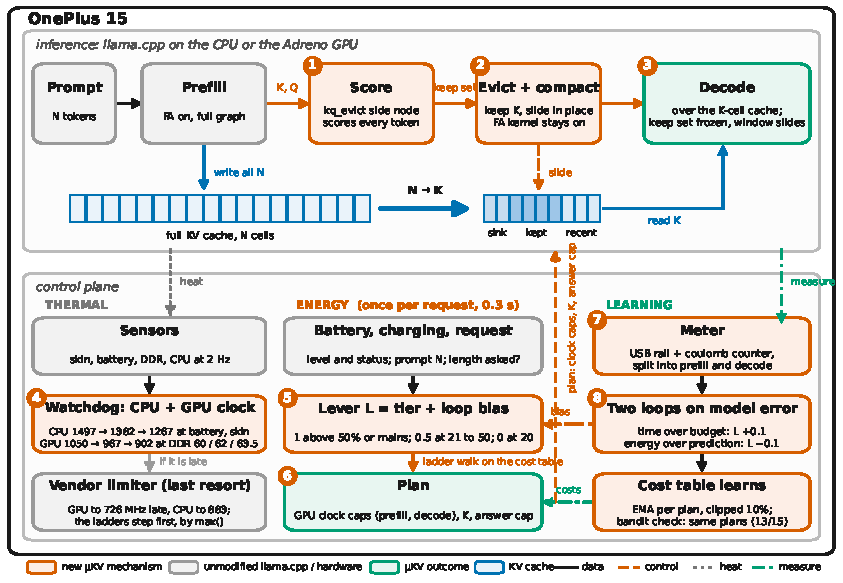
\includegraphics[width=0.94\textwidth]{figures/fig_architecture_v8.pdf}
\caption{$\mu$KV's pass. Scores come from a \texttt{kq\_evict} side node inside the FA-on prefill graph (+1.2\% prefill, paired $n{=}29$) --- a graph \emph{output}, immune by construction to the mid-graph interception that corrupts this backend. Selection produces one keep-set for all heads and layers; the in-place slide compacts survivors within prefill's own tensors, so peak memory never rises (the round-trip alternative is OS-killed at Phi-3/16K, on phone and on a 24\,GB RTX alike). The thermal/battery machinery is an independent outer loop that never touches the keep-set.}
\label{fig:architecture}
\end{figure*}

%% CHANGED 2026-08-17: fig_mechanism_v2 is a three-panel landscape redesign (the cell
%% array under each policy class, measured verdicts in the marks) -- it needs the full
%% text width; the old portrait flowchart it replaces fit one column.
\begin{figure*}[tb]
\centering
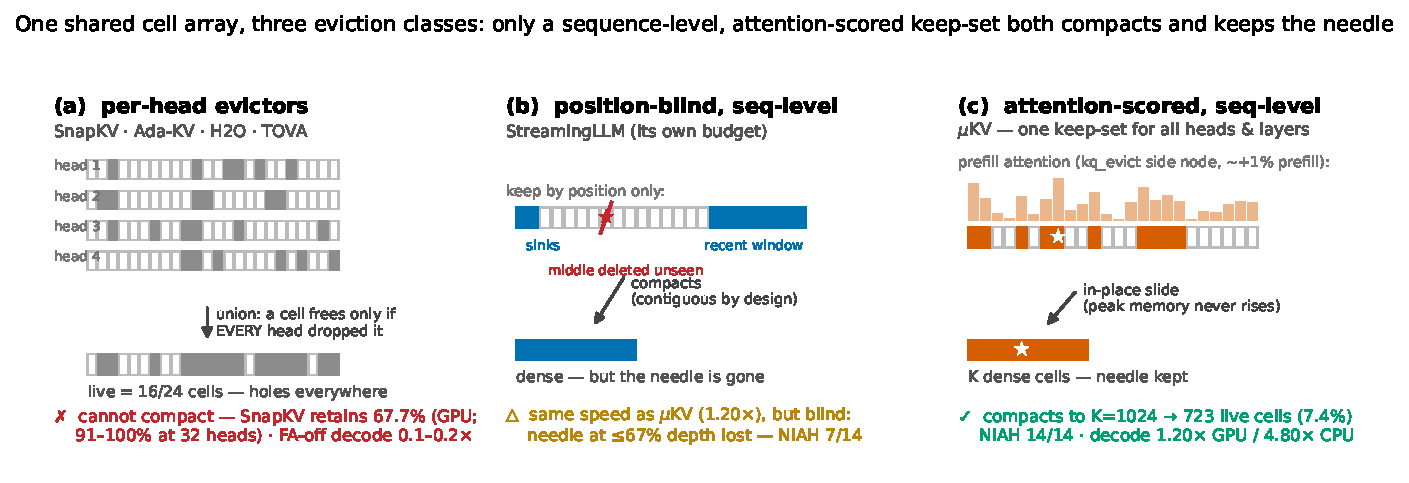
\includegraphics[width=0.97\textwidth]{figures/fig_mechanism_v2.pdf}
\caption{One shared cell array, three eviction classes. (a)~Per-head evictors union their keep-sets: SnapKV's budget of 1024 leaves 6592 cells live (67.7\%) --- the array cannot compact, and the FA-off decode path costs $5$--$10\times$. (b)~StreamingLLM at its own budget compacts by construction but deletes the middle unseen: every needle above its window-arithmetic depth cutoff is lost (7/14 measured; cutoffs 67\%/36\% at 8K/4K, observed exactly). (c)~$\mu$KV's single attention-scored keep-set compacts to 723 dense cells (7.4\%) and retrieves 14/14. Verdict lines are measured, not schematic.}
\label{fig:mechanism}
\end{figure*}


\textbf{Why the budget cannot come from the prompt.} The obvious rule is a ladder keyed on prompt length $N$. It fails in both directions. A 20-token instruction (``write a 2000-word report'') needs a \emph{large} budget, because the attended span grows during \emph{generation}, not during prefill; micro-budgets there backfire into repetition loops that emit more tokens~\cite{cai2025rkv}. A 10K-token retrieval prompt needs only a slice of $N$, since attention concentrates on a few heavy hitters~\cite{zhang2023h2o} and the query can be read from a prompt-end window~\cite{li2024snapkv}. Effective context is task-dependent, not length-dependent~\cite{hsieh2024ruler}. Figure~\ref{fig:kadaptive} measures this directly: break-even $K$ tracks \emph{output} length ($256\to4096$ as output grows $78\to2484$ tokens) and is flat in the 36-token prompt, where a length-keyed budget retrieves $0/5$ against a demand-aware one at $5/5$.

\emph{Why $K$ is the actuator.} Across our 372-cell dataset $K$ trades quality for both speed and heat: a larger resident cache lowers decode throughput ($r{=}{-}0.77$) and raises DDR temperature ($r{=}{+}0.80$), and higher temperature throttles throughput ($r{=}{-}0.71$). Over-provisioning $K$ wastes both; under-provisioning loses recall.

\emph{Demand-aware admission, then decode-time adaptation.} We keep $K$ as the actuator but re-found how it is chosen. At admission we size $K$ from the request's \emph{demand} rather than its input length: $K_\mathrm{init}$ is the larger of a retrieval floor $r(N)$ and a generation floor $g(\hat L_\mathrm{out},\text{task})$, clipped below by $K_\mathrm{min}$ and above by the thermal admission cap $K_\mathrm{tier}(T_\mathrm{DDR})$, where $r(N)$ covers the relevant prompt span, $g(\cdot)$ scales with the \emph{expected output length} $\hat L_\mathrm{out}$ (often user-declared, or estimable from task class), $K_\mathrm{min}\!\approx\!128$ guards the micro-budget backfire, and $K_\mathrm{tier}$ is the thermal admission cap. During decode $K$ grows as $\hat L_\mathrm{out}$ is revised upward and tightens when the model is confident, while the thermal ratchet supplies the downward term: demand raises $K$, heat lowers it.

\begin{figure}[tb]
\centering
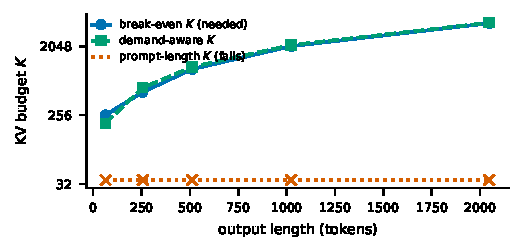
\includegraphics[width=0.92\columnwidth]{figures/fig_kadaptive.pdf}
\caption{Break-even budget $K$ scales with output length, not with the fixed 36-token prompt (controlled retention test, Llama-3.2-1B).}
\label{fig:kadaptive}
\end{figure}


Eviction is position-based, so filler is a faithful stand-in for generated tokens.


\textbf{per-head budget.} At end of prefill, for each head $h$ we read the last query's post-softmax attention $A_h$ and take its peak $m_h = \max_p A_h^p$. A sharp head (large $m_h$) needs few cells, a broad head more. We map $m_h$ through a closed-form ramp
\[
\begin{gathered}
\mu(x) = 1.3 - 0.6\cdot\mathrm{clip}\!\left(\tfrac{x-0.4}{0.4},0,1\right)\in[0.7,1.3],\\[2pt]
K_h = \mathrm{round}(K_{\text{nom}}\,\mu(m_h)),
\end{gathered}
\]
keeping the top $K_h$ positions per head, union over heads clipped to $K_{\text{nom}}$. This is $O(H)$ per layer against Ada-KV's $O(Hn\log Hn)$ global top-$B$ and needs no variable-length kernel. The breakpoints are therefore measured, but the clamp width is not: $[0.7,1.3]$ is a chosen $\pm30\%$ safeguard playing Ada-KV's $\alpha$-safeguard role so that no head starves or runs away. We did not sweep it --- the endpoints are compiled in --- and we make no claim that $\pm30\%$ is optimal. What we did sweep is the anchor:recent split $\alpha_a$, which the adaptive dispatcher now sets per prompt (\S\ref{sec:eval-cross}). The breakpoints 0.4 and 0.8 come from the measured $m_h$ distribution on Phi-3, where heads with $m_h>0.8$ are about 22\% of heads but 51\% of attention mass. The ramp is a cheap mobile approximation, not Ada-KV's optimal budget.

\textbf{adaptive-anchor dispatcher ($\alpha_a$).} The per-head gate candidate pool $\bigcup_h S_h$ must split into ``anchor'' (distant) and ``recent'' fractions. Rather than a hand-tuned constant, we compute a per-prompt $\alpha_a$ from the same prefill attention tensor the per-head gate used. Letting $\bar{\bar A}[p]$ be the column-mean over $(l, h)$, define $\mathrm{distant\_mass} = \sum_{p < N - R_\mathrm{min}} \bar{\bar A}[p]$ and $\mathrm{total\_mass} = \sum_p \bar{\bar A}[p]$. Then
\[
\boxed{\;\alpha_a = \mathrm{clip}\!\left(\frac{\mathrm{distant\_mass}}{\mathrm{total\_mass}},\, 0.05,\, 0.95\right)\;}
\]
sets $n_\mathrm{anchor} = \mathrm{round}(\alpha_a \cdot (K_\mathrm{nom} - n_\mathrm{sink}))$ and $n_\mathrm{recent} = K_\mathrm{nom} - n_\mathrm{sink} - n_\mathrm{anchor}$. The cost is one column-mean reduction, the same reduction anchor selection already needs, so the dispatcher adds zero forward passes. Empirically (\S\ref{sec:eval-cross}, the mass-$\alpha_a$ ablation) $\alpha_a$ varies per prompt (0.62--0.95), auto-discovering the throughput corner on chat prompts and the quality corner on retrieval prompts without a deploy-time hyperparameter.

\textbf{selective anchoring.} The per-head union can retain hundreds of prompt cells and starve the recent window. We re-rank the union by mean cross-head attention and keep only the top $n_\mathrm{anchor}$ (from the dispatcher) as anchors, plus 4 sink tokens~\cite{xiao2024streamingllm}, leaving $n_\mathrm{recent}$ for the recent window. Without this cap, Phi-3 perplexity spiked to 158 in early runs.

\textbf{cache precision.} K is quantized to q8\_0, V kept at f16, a lighter profile than KIVI's 2-bit scheme~\cite{liu2024kivi} and free of training. This halves the K-side read and drops DDR temperature by about 3\,\textdegree C on Phi-3. On small models the dequantize cost can exceed the bandwidth saving, so it pays only above roughly 1\,GB cache (\S\ref{sec:eval-cross}).

\textbf{fast-path scoring and compaction.} The gate and dispatcher need post-softmax attention, which historically forced the slow FA-off path during prefill. $\mu$KV instead computes the scores inside the FA-on prefill graph through a small \texttt{kq\_evict} side node emitted only on the last prefill chunk (earlier chunks' scores are overwritten anyway), so selection is bit-identical and prefill costs the same as vanilla. An \emph{in-place} pass then slides the survivors into a dense prefix inside the tensors prefill already allocated, over which decode runs FA-on; peak memory never rises. (The earlier serialize-and-restore round-trip needs a second full cache: at Phi-3/16K it is OS-killed on the phone and fails identically on a 24\,GB RTX~4500, so in-place is what makes that configuration feasible at all. The two modes select identical cells --- verified to 0.15\% PPL across a three-way check at 64K.) An earlier variant captured scores from an FA-off prefill and swapped the compacted cache into an FA-on context to decode. It selects the same cells but costs 10--15\% more prefill, and it is superseded by the side node; we do not report it as a configuration. During decode a tiered re-eviction fires only when the active cache exceeds $1.25\times(n_{\text{anchor}}+B_R)$, amortizing eviction across many steps.

\textbf{watchdog.} A separate process samples DDR, CPU big-core, skin, battery temperature, and battery current at 2\,Hz, computes a per-sensor threat as the clamped warn-to-crit fraction, and takes the maximum. It lowers the big-core frequency cap one step at a time along direct temperature ladders anchored at the \emph{measured} deep-throttle trigger (battery 47.0\slb48.0\slb48.5\slb49.0\slb49.5\,\textdegree C and skin 50.0\slb51.0\slb51.5\slb52.0\slb52.5\,\textdegree C map to 1497\slb1382\slb1267\slb1132\slb1017\,MHz; DDR is a backstop only above 71\,\textdegree C, as it runs 66--69\,\textdegree C normally here), stepping down as thresholds approach and never rising above base, so it can only reduce. The thresholds are calibrated from the trigger we measured, not chosen in theory: on this SoC the vendor deep-throttle fires the instant battery reaches 50\,\textdegree C (Sec.~\ref{sec:eval-thermal}), and the ladder glides the clock below the vendor clamp through the 47--49\,\textdegree C run-up, with a 1017\,MHz floor above the 883\,MHz cliff. %% MEASURED 2026-08-17 (8-generation soak, Aug 9, post zone-fix): the claim is now the
%% residency number, not "holds the battery below 50 C" -- peak is UNCHANGED across arms;
%% what changes is how long the device sits on the throttle floor.
On a cold phone it stays dormant. Measured over an 8-generation soak it cuts time below 500\,MHz from 41.0\% to 28.5\% of the run, at $+3.6^\circ$C mean DDR and \emph{unchanged} peak DDR ($\sim$78.5\,\textdegree C on every arm): it keeps the device off the throttle floor rather than lowering the ceiling (Fig.~\ref{fig:bonsai-thermal}). The watchdog acts on one actuator: \emph{CPU frequency}.

\paragraph{Cost model.} Per decode step the wall time is bandwidth-bound: it scales with bytes read per step, set by the resident cache size and DDR bandwidth, the latter falling as DDR heats (the LPDDR5X refresh interval doubles near 85\,\textdegree C). Shrinking $K$ cuts bytes per step and so cuts both time and energy, but does not cap peak temperature: under sustained load frequency is the only lever that does (\S\ref{sec:eval-tdak}), which is why the watchdog acts on the clock and eviction on efficiency.
\paragraph{Three reductions of the same attention tensor.} The per-head gate, dispatcher, and anchor selection each take a \emph{different} reduction axis through the same captured tensor $\bar A_{l,h,p}$; none duplicates another:
\begin{itemize}[leftmargin=*, itemsep=2pt]
\item \textbf{the per-head gate (per-head row-max)} $\to$ per-head budget $K_h$: $m_h = \max_p \bar A_{l,h,p}$, then $K_h = \mathrm{round}(K_\text{nom}\cdot\mu(m_h))$.
\item \textbf{the dispatcher (cross-head column-mean partition)} $\to$ per-prompt anchor:recent split $\alpha_a$: $\bar{\bar A}[p] = \frac{1}{n_\text{layers}\,n_\text{heads}}\sum_{l,h} \bar A_{l,h,p}$, then $\alpha_a = \mathrm{distant\_mass}/\mathrm{total\_mass}$.
\item \textbf{anchor selection (column-mean top-K)} $\to$ which positions survive: $\mathrm{Anchor} = \mathrm{TopK}_{n_\text{anchor}}(\bar{\bar A})$.
\end{itemize}
The kept set is then $K = n_\text{sink} + n_\text{anchor} + n_\text{recent}$ with $n_\text{anchor} = \alpha_a(K-n_\text{sink})$ and the remainder a sliding recent window, so a reported budget of $K{=}1024$ means 4 sinks plus, e.g., 721 anchors and 299 recent, not 1024 anchors. Crucially this is \emph{one shared set across all heads}, which is what lets $\mu$KV compact on a sequence-level engine where per-head evictors cannot.
All three share the same $\bar A$ already captured for FA-off prefill, so no extra forward pass is needed.

\section{Evaluation}
\label{sec:eval}

\textbf{Setup.} OnePlus 15, Snapdragon 8 Elite Gen 5, 12\,GB UMA, CPU-only, 4 threads. Models: Phi-3-mini-128k, Llama-3.2-1B, gemma-2-2b-it, all Q4\_K\_M, run in a \texttt{llama.cpp} extension~\cite{llamacpp} we call \texttt{eviction\ub bench}. Each cell starts from a verified cool baseline (DDR/CPU $<$\,40\,\textdegree C; skin/PMIC/battery $<$\,36\,\textdegree C); USB charging is held OFF continuously by a per-cell keeper that re-disables every 30\,s (Android battery service otherwise re-enables charging mid-run). Per-cell sensor capture at 5\,Hz, with USB rail $V{\cdot}I$ integration for true system energy (\texttt{usb\_current\_ua}, \texttt{usb\_voltage\_uv}). $\mu$KV runs with mass-based $\alpha_a$ and the multi-sensor watchdog; baselines run as published.

\textbf{Two benchmarks at the same 16K context.}
\emph{(1) Sustained decode} (Table~\ref{tab:master-wikitext}). A $\sim$7K-token prompt (7.5K Phi-3 / 6.4K Llama-1B / 6.4K Gemma-2B) followed by 2K-token greedy generation with \texttt{-{}-ignore\allowbreak-eos}, in a 16{,}384-token allocated context (hence ``16K'' = KV-cache allocation, not prompt length). One run per (policy, model) cell. Measures the systems axes: throughput (decode tps), peak DDR/CPU/skin/PMIC/battery temperature, USB-rail energy, peak RSS, plus PPL on the decoded text. This is the workload that exposes thermal-cliff behavior because it sustains pressure for $\sim$10--50 minutes per cell.
\emph{(2) RULER-style NIAH retrieval} (Table~\ref{tab:phone-niah-prelim}). A buried-fact prompt: $\sim$5K--16K tokens of filler with the needle ``mango sorbet at Bi-Rite Creamery is the best thing to do in San Francisco'' inserted at one of 7 depths ($\{0, 17, 33, 50, 67, 83, 100\}\,\%$ of context), followed by ``Q: What's the best thing to do in SF?''. One run per (policy, model, context, depth). \emph{Hit} = generated text contains ``mango sorbet'' or ``bi-rite'' (case-insensitive). Measures the quality axis: can the policy retrieve a buried fact regardless of where it sits in the prompt? Total: 7 policies $\times$ 4 models $\times$ 14 depths (7 at 4K + 7 at 8K) $= 392$ cells, \textbf{all complete}. A hit means the generation names the needle as an answer; a generation that denies the fact and then mentions the phrase is scored a miss, which a plain substring match over-counts.

\emph{Why both?} 16K-decode catches policies that fail thermal sustainability (slow or hot under long generation); NIAH catches policies that achieve speed by dropping information (StreamingLLM-style sliding window, which sweeps 16K-decode but fails NIAH because the needle gets evicted). Only a policy that wins BOTH benchmarks is deployable.



\begin{table*}[tp]
\caption{\textbf{WikiText sustained decode, phone CPU --- every policy, one build, cold start per cell.}
9.7K-token prompt $+$ 4K greedy decode, 16K context, Llama-3.2-1B Q4\_K\_M, 6 threads, cool gate
(CPU/DDR $<$37\,\textdegree C, shell $<$34\,\textdegree C, start temperatures recorded per cell), charging
held off throughout, energy $=$ USB-rail integral $+$ coulomb counter. Each baseline at its own published
configuration. ActKV is retained \emph{live} cells; \emph{italic} marks a nominal budget that failed to
materialise. PPL$_\text{rec}$ is teacher-forced on a slice that \emph{overlaps} the prompt, so it scores
verbatim recall of retained text and tracks retention ($r{=}{-}0.96$ vs.\ live cells) --- it ranks how much
prompt survived, not quality, and must not be read as an eviction-quality metric (\S\ref{sec:eval-cross}).
$^{*}$the same $\mu$KV configuration measured on the earlier bin\_cpu\_sol2 build, retained because it is an independent measurement of the headline row: 24.21 vs.\ 23.15\,tok/s, a 4.4\% spread at $n{=}1$ per cell. \textbf{All energies in this table use one pipeline} (whole-run, rail $+$ coulomb). Earlier drafts quoted energies from a different script that we can no longer reproduce from the raw traces --- they sat between the whole-run and decode-only windows with no consistent rule. The \emph{ratio} is unaffected and is what we claim: $\mu$KV uses $58$--$62\%$ less energy than the full cache under every method tried (published 0.379, prior build 0.396, this build 0.415). Vanilla reproduces 5.02\,tok/s on both builds.}
\label{tab:master-wikitext}
\centering\small
\setlength{\tabcolsep}{5pt}
\begin{tabular}{l l r r r r r r r}
\toprule
\textbf{Policy} & \textbf{Config} & \textbf{PPL$_\text{rec}$} & \textbf{tok/s} & \textbf{$\times$van}
 & \textbf{Prefill\,(s)} & \textbf{Wall\,(s)} & \textbf{ActKV} & \textbf{Energy\,(mWh)} \\
\midrule
\textbf{$\mu$KV} & wd off & 8.23 & \textbf{23.40} & \textbf{4.66} & 187 & \textbf{362} & \textbf{721} & \textbf{601} \\
$\mu$KV          & wd on  & 8.23 & 23.15 & 4.61 & 232 & 409 & 721 & 641 \\
$\mu$KV$^{*}$    & wd on, prior build & 8.03 & 24.21 & 4.82 & 226 & 396 & 721 & 522 \\
KeyDiff          & K=2048 & 1.99 & 17.36 & 3.46 & 195 & 431 & 2049 & 738 \\
Ada-KV           & FA \textbf{on} & 2.60 & 11.52 & 2.29 & 210 & 566 & 3489 & 845 \\
KeyDiff          & K=4096 & 1.42 & 10.78 & 2.15 & 198 & 578 & 4098 & 853 \\
KeyDiff          & K=6144 & 1.15 & 8.02 & 1.60 & 202 & 713 & 6146 & 1025 \\
SnapKV           & FA off & 1.67 & 6.83 & 1.36 & 250 & 849 & 5931 & 1180 \\
Ada-KV           & FA off & 2.63 & 6.79 & 1.35 & 253 & 856 & 3485 & 1194 \\
H2O              & FA off & 4.53 & 6.45 & 1.29 & 221 & 856 & \textit{9151} & 1262 \\
KeyDiff          & K=8192 & 1.07 & 6.43 & 1.28 & 175 & 812 & 8195 & 1261 \\
TOVA             & FA off & 4.53 & 5.92 & 1.18 & 225 & 917 & 4093 & 1200 \\
SnapKV           & FA \textbf{on} & 1.12 & 5.38 & 1.07 & 192 & 953 & \textit{8893} & 1346 \\
vanilla          & full cache & 1.06 & 5.02 & 1.00 & 181 & 996 & 9741 & 1544 \\
\bottomrule
\end{tabular}
\end{table*}




\paragraph{Measurement protocol.}\label{sec:revised-protocol}
All cells run on one build (aarch64, armv8.7-a with i8mm and repack kernels) so throughput is comparable across policies. The vendor DVFS and thermal engine govern every cell from a cold start (CPU and DDR below 37\,\textdegree C, shell below 34\,\textdegree C); we impose no frequency cap. Under sustained bandwidth-bound decode the vendor clamps \texttt{scaling\ub max} to ${\sim}1632$\,MHz, and to ${\sim}1498$\,MHz once skin passes 41\,\textdegree C. That clamp is temperature-set and identical for all policies, so the clock is not a confound. Charging stays disabled so the state of charge is constant, and energy integrates total system power split at the prefill/decode boundary. Retained KV is measured by \texttt{llama\ub state\ub seq\ub get\ub size}, which serializes live cells only; position-range counters over-state it. Every baseline runs its own paper's configuration with none of $\mu$KV's mechanisms: SnapKV uses the FasterDecoding defaults (window 64, avgpool-5, no sinks); Ada-KV the Ada-SnapKV defaults (window 32, maxpool-7, $\alpha{=}0.2$ safeguard); H2O its 50/50 heavy-hitter and recent split; StreamingLLM 4 sinks plus a recent window; TOVA its paper-preferred per-layer form scoring from the last query. The watchdog runs on $\mu$KV only and stays dormant from cold. Table~\ref{tab:master-wikitext} reports this workload as a 9.7K-token prompt followed by 4K greedy decode at nominal $K{=}1024$. PPL$_\text{rec}$ is teacher-forced perplexity on an eval slice that \emph{overlaps} the prompt, so it scores verbatim recall of retained text rather than prediction; on a disjoint slice every policy matches the full cache. ActKV is retained live KV cells, with the $\mu$KV decode-mean in parentheses. Per-head policies cannot compact on a sequence-level engine, so their ActKV stays high.

Two caveats. First, the PPL$_\text{rec}$ column measures recall, not quality, which is why we renamed it. Its evaluation text overlaps the prompt, so a policy that keeps the prompt can copy the answer. Vanilla's 1.06 is recall, not quality: holding the full context, it recognizes the passage and reproduces it. $\mu$KV's 8.23 is what a Llama-class model scores when it must actually predict. The column therefore ranks policies by how much prompt they retained, which is the thing under test.

We re-ran the measurement with the confound removed, on a WikiText slice verified disjoint from the prompt (0 of 159 sliding 200-character probes appear in it). On that slice $\mu$KV matches the full cache on every healthy configuration, after evicting about 92\% of the prompt cache:

On that slice $\mu$KV matches the full cache within 2\% on every healthy configuration after evicting about 92\% of the prompt cache: Llama-3.2-1B Q8\ub 0 8.198 vs 8.023, Phi-3-mini Q4\ub K\ub M 3.983 vs 3.938 (both GPU-resident), and the 1-bit Bonsai-8B 6.717 vs 6.736.

\noindent So eviction does not cost language-modeling quality. What it costs is verbatim recall of the spans it drops --- exactly what the overlapping-slice number measured and what NIAH probes. Self-generation PPL is about 1.1 for every policy. We keep the recall column for continuity with prior work, which reports perplexity in this overlapping form, but treat the disjoint slice and NIAH accuracy as the quality result. A second caveat: $\mu$KV's decode-time eviction bounds the cache near 2K cells, above the nominal $K{=}1024$, while every baseline grows without bound; we report the measured mean, not the nominal budget.

\paragraph{Reading the figures.} The mechanism is a compaction step: every policy builds the full prompt cache during prefill; at its end $\mu$KV compacts to 721 anchors (its $K{=}1024$ splits into 4 sinks, 721 score-selected anchors, and a 299-token recent window) and decode-time eviction keeps the cache bounded near 2K, while SnapKV drops only to 5.9K and vanilla grows without bound. Table~
ef{tab:master-wikitext} shows what that buys. Neither policy's clock explains it --- both run at ${\sim}1.6$\,GHz. The heat source shifts: the CPU is hot during compute-bound prefill, the DRAM during memory-bound decode. $\mu$KV's 13$\times$ smaller cache (23 vs.\ 304\,MiB) moves far less I/O, so DDR peaks ${\sim}5$\,\textdegree C cooler and it finishes in 6.6 vs.\ 17.4 minutes. Memory traffic drives both the speed and the thermal win.

% auto-generated by scripts/make_gpu_table.py -- do not hand-edit
% auto-generated by scripts/make_gpu_table.py -- do not hand-edit
% auto-generated by scripts/make_gpu_table.py -- do not hand-edit
\begin{table}[tb]
\caption{Mobile GPU (Adreno 840): 12K-token WikiText prompt $+$ 4096 generated $=$ the full 16384 context, batch 1, cold-start gate (DDR $\le35$\,\textdegree C, battery $\le33$\,\textdegree C) before every cell. \textbf{f16 K/V for every policy}: quantized KV is numerically broken on this Adreno build (the model emits random tokens; teacher-forced NLL exceeds $\ln(\text{vocab})$), and f16 is in any case the only format all policies can share, since a per-head evictor needs FA-off and llama.cpp requires flash-attention for a quantized V. Values are the median of $n$ runs with the range in brackets. \textbf{Cells} is retained cache in KV cells, invariant to cache format. Phi-3 $\mu$KV is reported at ctx 8192: compaction restores into a \emph{second} context, so its peak demand is twice the cache, and at 16K in f16 that is $2\times6.44+2.4=15.28$\,GB against 15.1\,GB of phone RAM --- every 16K Phi-3 cell records compaction\ub applied=False. Llama-1B needs only 1.87\,GB and compacts at 16K. This is the same 2$\times$ round-trip bound that limits compaction at 64K on the RTX.}
\label{tab:gpu-wikitext}
\centering\small
\setlength{\tabcolsep}{4pt}
\begin{tabular}{l l r r r r r}
\toprule
\textbf{Model} & \textbf{Policy} & \textbf{$n$} & \textbf{Prefill} & \textbf{tok/s} & \textbf{dec\,$\times$} & \textbf{Cells} \\
\midrule
\multicolumn{7}{l}{\emph{Llama-3.2-1B}} \\
  & vanilla (full cache)     & 3 & 124 & 24.28 $\pm$ 0.12 & 1.00$\times$ & 9741 \\
  & \textbf{$\mu$KV}         & 3 & 138 & 29.77 [29.3--39.5] & 1.23$\times$ & 723 \\
  & $\mu$KV, no compaction   & 3 & 132 & 25.61 [25.6--25.8] & 1.06$\times$ & 723 \\
  & SnapKV                   & 1 & 229 & 4.76 & 0.20$\times$ & 6592 \\
  & Ada-KV                   & 1 & 276 & 2.86 & 0.12$\times$ & 3519 \\
  & TOVA                     & 1 & 176 & 4.34 & 0.18$\times$ & 4125 \\
  & H2O                      & 1 & 279 & 3.58 & 0.15$\times$ & 6110 \\
  & StreamingLLM (own budget)$^{\ddagger}$ & 3 & 125 & 29.07 $\pm$ 0.18 & 1.20$\times$ & 2005 \\
  & \emph{--- as our earlier tables ran it}$^{\S}$ & 1 & 234 & 5.75 & 0.24$\times$ & 777 \\
\midrule
\multicolumn{7}{l}{\emph{Phi-3-mini}} \\
  & vanilla (full cache)     & 3 & 606 & 4.27 [4.2--4.4] & 1.00$\times$ & 11157 \\
%% CORRECTED 2026-08-17: "does not fit" was true only of the round-trip mechanism;
%% in-place compaction runs this configuration (reproduced; the round-trip is the
%% thing that is OS-killed, on phone AND on a 24 GB RTX).
  & \textbf{$\mu$KV (in-place)} & 3 & 694 & 12.00 & 2.81$\times$ & 874 \\
  & $\mu$KV, no compaction   & 3 & 621 & 8.78 [8.1--8.8] & 2.06$\times$ & 878 \\
  & SnapKV                   & 1 & 966 & 0.91 & 0.21$\times$ & 9468 \\
  & Ada-KV                   & 1 & 923 & 1.27 & 0.30$\times$ & 3796 \\
  & TOVA                     & 1 & 853 & 1.19 & 0.28$\times$ & 5252 \\
  & H2O                      & 1 & 1078 & 1.04 & 0.24$\times$ & 10095 \\
  & StreamingLLM             & 1 & 830 & 1.20 & 0.28$\times$ & 917 \\
\midrule
\midrule
\multicolumn{7}{l}{\emph{Phi-3-mini, ctx 8192 --- the largest context where compaction fits (see caption)}} \\
  & vanilla (full cache)     & 3 & 157 & 7.59 [7.3--8.6] & 1.00$\times$ & 4091 \\
  & \textbf{$\mu$KV}         & 3 & 160 & 13.59 [13.5--14.3] & 1.79$\times$ & 885 \\

\multicolumn{7}{l}{\footnotesize $^{\ddagger}$pinned protocol (taskset+nice, cool-gated, $n{=}3$); $^{\S}$our earlier handicapped configuration --- FA off, uncompacted, half its}\\
\multicolumn{7}{l}{\footnotesize published budget --- kept so the size of our own error stays measured (its output is also invalid on this backend, \S\ref{sec:eval-cross}).}\\
\bottomrule
\end{tabular}
\end{table}

\begin{table*}[tb]
\caption{Phone NIAH retrieval: hits out of 7 needle depths per block. All 392 cells share one build, ctx 16384 and the cold-start gate. Retained-cache figures are reported per model in \S\ref{sec:eval}, not averaged here: Phi-3's per-token KV is 24$\times$ Llama-1B's, so a single mean across models would describe our model mix rather than the policy.}
\label{tab:phone-niah-prelim}
\centering\small
\setlength{\tabcolsep}{5pt}
\begin{tabular}{l cc cc cc cc r}
\toprule
& \multicolumn{2}{c}{Phi-3} & \multicolumn{2}{c}{Llama-1B} & \multicolumn{2}{c}{Gemma-2B} & \multicolumn{2}{c}{Bonsai-8B} & \\
\cmidrule(lr){2-3}\cmidrule(lr){4-5}\cmidrule(lr){6-7}\cmidrule(lr){8-9}
\textbf{Policy} & 4K & 8K & 4K & 8K & 4K & 8K & 4K & 8K & \textbf{Total} \\
\midrule
vanilla (full cache) & 7 & 7 & 7 & 6 & 6 & 5 & 7 & 7 & 52/56 \\
\textbf{$\mu$KV} & \good{7} & \good{7} & \good{7} & \good{6} & \good{6} & \good{5} & \good{7} & \good{7} & \good{52/56} \\
SnapKV & 7 & 7 & 7 & 5 & 6 & 5 & 7 & 7 & 51/56 \\
AdaKV & 7 & 7 & 7 & 5 & 6 & 5 & 7 & 7 & 51/56 \\
TOVA & 7 & 7 & 7 & 5 & 6 & 5 & 7 & 7 & 51/56 \\
H2O & 7 & 7 & 6 & \bad{2} & 6 & \bad{4} & 7 & 6 & \bad{45/56} \\
StreamingLLM & \bad{2} & \bad{1} & \bad{2} & \bad{1} & \bad{1} & \bad{1} & \bad{2} & \bad{1} & \bad{11/56} \\
\bottomrule
\end{tabular}
\end{table*}

% auto-generated by scripts/make_longbench_table.py -- do not hand-edit
\begin{table*}[tb]
\caption{LongBench F1 (official token-F1, max over reference answers) on the RTX 4500 Ada. Every policy runs f16 K/V here, so F1 and retained cache are quantization-matched: SnapKV cannot use quantized KV on this engine at all, since a per-head evictor needs FA-off and llama.cpp requires flash-attention for a quantized V. \textbf{Cells} is retained cache in KV cells (format-independent) as a percentage of the prompt. SnapKV runs its published LongBench configuration (window 32, avgpool-7); its NIAH setting (16/5) and the FasterDecoding default (64/5) were also measured and span only 0.8 F1 on Llama-1B, so the comparison does not turn on that choice. Gemma-2-2B runs at ctx 8192, its trained context; the other models at 16384. $^{\dagger}$StreamingLLM runs its OWN published budget, \texttt{start\_size}~4 + \texttt{recent\_size}~2000 = 2004 cells (its repository's argparse defaults), not the $K{=}1024$ every other row uses. An earlier version of this table ran it at 1024 --- roughly half the cache its authors specify --- which cost it 1.7--4.6 F1 and reported it at $-6.1/-7.4/-10.8/-9.6$ instead of the $-4.4/-4.2/-6.2/-7.4$ here. Its retained cells rise correspondingly, so it is no longer at $\mu$KV's retention: $\mu$KV holds $2.4\times$ less cache and still scores 4--7 F1 higher. Re-measured 2026-08-16, same 50 samples, same prompts, same binary; only \texttt{--k-nominal} changed.}
\label{tab:longbench}
\centering\small
\setlength{\tabcolsep}{5pt}
\begin{tabular}{l l r r r r r  r r}
\toprule
\textbf{Model} & \textbf{Policy} & \textbf{HotpotQA} & \textbf{2WikiMQA} & \textbf{MultiFieldQA} & \textbf{Qasper} & \textbf{TriviaQA} & \textbf{Avg} & \textbf{Cells kept} \\
\midrule
\multicolumn{9}{l}{\emph{Llama-1B\ \ (ctx 16384)}} \\
  & vanilla (full cache)       & 42.14 & 23.86 & 45.04 & 17.55 & 81.19 & 41.96 & 8687 (100.0\%) \\
  & \textbf{$\mu$KV}           & 40.72 & 25.53 & 43.23 & 17.06 & 83.88 & 42.08 (+0.1) & 826 (13.0\%) \\
  & SnapKV                     & 41.14 & 23.51 & 45.02 & 22.81 & 81.19 & 42.73 (+0.8) & 6717 (82.4\%) \\
  & Ada-KV                     & 41.84 & 22.17 & 46.16 & 22.10 & 81.19 & 42.70 (+0.7) & 3327 (47.3\%) \\
  & TOVA                       & 41.61 & 22.98 & 45.62 & 21.93 & 81.86 & 42.80 (+0.8) & 3824 (53.5\%) \\
  & H2O                        & 42.68 & 24.04 & 41.87 & 19.35 & 81.20 & 41.83 (-0.1) & 6699 (83.1\%) \\
  & StreamingLLM$^{\dagger}$   & 35.61 & 18.14 & 36.52 & 16.51 & 81.00 & 37.56 (-4.4) & 1994 (23.0\%) \\
\midrule
\multicolumn{9}{l}{\emph{Gemma-2B\ \ (ctx 8192)}} \\
  & vanilla (full cache)       & 46.51 & 34.51 & 45.19 & 36.42 & 87.67 & 50.06 & 6457 (100.0\%) \\
  & \textbf{$\mu$KV}           & 40.32 & 37.20 & 39.63 & 31.71 & 87.67 & 47.31 (-2.8) & 716 (13.0\%) \\
  & SnapKV                     & 40.51 & 36.81 & 45.40 & 38.38 & 87.44 & 49.71 (-0.4) & 6031 (94.2\%) \\
  & Ada-KV                     & 40.51 & 36.81 & 44.55 & 37.26 & 87.44 & 49.31 (-0.7) & 4064 (66.3\%) \\
  & TOVA                       & 41.52 & 37.31 & 44.37 & 37.45 & 87.44 & 49.62 (-0.4) & 4087 (66.9\%) \\
  & H2O                        & 37.38 & 37.31 & 43.61 & 35.37 & 87.44 & 48.22 (-1.8) & 5869 (92.1\%) \\
  & StreamingLLM$^{\dagger}$   & 41.51 & 32.67 & 38.72 & 28.59 & 87.67 & 45.83 (-4.2) & 1995 (30.9\%) \\
\midrule
\multicolumn{9}{l}{\emph{Phi-3\ \ (ctx 16384)}} \\
  & vanilla (full cache)       & 46.86 & 43.51 & 57.05 & 36.92 & 87.87 & 54.44 & 9702 (100.0\%) \\
  & \textbf{$\mu$KV}           & 45.97 & 43.18 & 55.85 & 40.80 & 86.37 & 54.43 (-0.0) & 853 (12.2\%) \\
  & SnapKV                     & 46.85 & 40.01 & 55.62 & 38.35 & 87.20 & 53.61 (-0.8) & 7629 (83.4\%) \\
  & Ada-KV                     & 46.90 & 38.48 & 56.51 & 37.33 & 87.87 & 53.42 (-1.0) & 4056 (50.6\%) \\
  & TOVA                       & 54.81 & 38.67 & 55.33 & 50.60 & 87.87 & 57.45 (+3.0) & 4550 (54.9\%) \\
  & H2O                        & 48.32 & 39.66 & 56.12 & 36.97 & 88.20 & 53.85 (-0.6) & 8702 (91.2\%) \\
  & StreamingLLM$^{\dagger}$   & 40.71 & 41.88 & 40.05 & 30.68 & 87.87 & 48.24 (-6.2) & 1999 (20.6\%) \\
\midrule
\multicolumn{9}{l}{\emph{Bonsai-8B\ \ (ctx 16384)}} \\
  & vanilla (full cache)       & 35.11 & 33.39 & 50.03 & 38.53 & 86.15 & 48.64 & 8928 (100.0\%) \\
  & \textbf{$\mu$KV}           & 35.16 & 24.33 & 48.13 & 32.30 & 84.95 & 44.97 (-3.7) & 797 (12.6\%) \\
  & SnapKV                     & 38.58 & 34.30 & 50.12 & 38.59 & 88.15 & 49.95 (+1.3) & 8716 (96.1\%) \\
  & Ada-KV                     & 34.46 & 34.48 & 50.75 & 37.56 & 87.48 & 48.95 (+0.3) & 5293 (68.2\%) \\
  & TOVA                       & 37.06 & 30.19 & 50.76 & 37.88 & 87.48 & 48.67 (+0.0) & 5700 (72.5\%) \\
  & H2O                        & 36.66 & 28.54 & 49.03 & 34.97 & 88.15 & 47.47 (-1.2) & 7798 (90.9\%) \\
  & StreamingLLM$^{\dagger}$   & 34.40 & 24.97 & 30.13 & 30.24 & 86.26 & 41.20 (-7.4) & 2246 (25.2\%) \\
\midrule
\bottomrule
\end{tabular}
\end{table*}

% ============================================================================
% tab_related_mobile.tex -- what mobile KV-cache work has ACTUALLY measured.
%                           (2026-08-03)
%
% Every row was verified from the paper's own evaluation section, not its
% abstract or title -- because the titles are systematically misleading here.
% Two papers branded "mobile" (KVSwap, MobiLoRA -- the latter co-authored with a
% phone vendor) evaluate on Jetson boards; MobiLoRA calls the AGX Orin "the
% widely used mobile development platform". KeyDiff's only phone result is a
% normalized scoring-kernel microbenchmark in Appendix H.4. DynaKV's four
% OnePlus devices are real, but it is CPU-only and lists GPU as future work.
%
% The table exists to support one narrow, checkable claim: KV-cache EVICTION has
% never been deployed end-to-end on a smartphone GPU. It is not a quality
% ranking -- several of these systems are excellent at what they do.
% ============================================================================
\begin{table*}[tb]
\caption{Mobile KV-cache work: what each paper \emph{measured}, verified from its evaluation section rather than its title. The field splits cleanly: policies that \emph{evict} run on servers or Jetson-class boards; systems that run on \emph{phones} keep every token (offload, reuse, or quantize); and studies that do use a phone \emph{GPU} apply no cache management at all. $\mu$KV occupies the empty cell.}
\label{tab:related-mobile}
\centering\small
\setlength{\tabcolsep}{4pt}
\begin{tabular}{l l l c l l}
\toprule
\textbf{System} & \textbf{Venue/yr} & \textbf{Hardware evaluated on} & \textbf{Phone} & \textbf{Compute used} & \textbf{KV mechanism} \\
\midrule
\multicolumn{6}{l}{\emph{KV eviction, but never on a phone}} \\
SnapKV, Ada-KV, H2O, TOVA, PyramidKV & '23--'24 & A100-class servers & \no & server GPU & eviction \\
KVSwap & MobiSys'25 & Jetson Orin AGX 64\,GB $+$ NVMe & \no & board GPU & offload to disk \\
MobiLoRA & ACL'25\rlap{$^{\dagger}$} & NVIDIA AGX Orin & \no & board GPU & cache reuse \\
KeyDiff & NeurIPS'25\rlap{$^{\ddagger}$} & A100 80GB; unnamed Samsung phone (App.~H.4) & \yes\rlap{$^{\S}$} & \textbf{not stated} & eviction \\
\midrule
\multicolumn{6}{l}{\emph{On a real phone, but never eviction --- and never the GPU}} \\
DynaKV & 2025\rlap{$^{\dagger}$} & OnePlus Ace5\,Pro / 12 / Ace3 / Ace2 & \yes & \textbf{CPU only}\rlap{$^{\P}$} & offload to UFS \\
ActiveFlow & 2025 & OnePlus 12, Pixel 6, Infinix ZERO 30 & \yes & \textbf{CPU only} & weights, not KV \\
PowerInfer-2 & MobiSys'25 & OnePlus 12, OnePlus Ace 2 & \yes & CPU $+$ NPU & neurons, not KV \\
PerCache & 2026 & Pixel 7, Redmi K60 Pro, S22 Ultra, Ace 6 & \yes & not stated & QKV reuse (RAG) \\
Persistent Q4 KV & 2026 & MacBook Pro M4 Pro & \no & Metal & quantize $+$ persist \\
\midrule
\multicolumn{6}{l}{\emph{On a phone GPU, but no cache management at all}} \\
LLMs in Your Pockets & 2026 & 7 devices: Adreno 750/730, Mali-G720/G78 & \yes & CPU, GPU, NPU & \textbf{none} \\
LLM Inference at the Edge & 2026 & S24 Ultra (Adreno 750), iPhone 16 Pro & \yes & \textbf{GPU} & \textbf{none} \\
\midrule
\textbf{$\mu$KV (this work)} & --- & \textbf{OnePlus 15, Adreno 840} & \yes & \textbf{CPU and GPU} & \textbf{eviction $+$ compaction} \\
\bottomrule
\end{tabular}

\vspace{2pt}
{\footnotesize $^{\dagger}$co-authored with Honor Device Co. \quad $^{\ddagger}$Qualcomm AI Research. \quad
$^{\S}$every model result (LongBench, NIAH, and the headline 30\% end-to-end TTFT gain) is measured on A100; the phone appears only in App.~H.4, which reports five \emph{normalized} ratios for the eviction-\emph{scoring kernel} --- no model is run on the device, and no absolute latency, throughput, footprint or energy is given. \quad
$^{\P}$``we adopt the CPU as the primary backend''; CPU--GPU is Discussion~2, future work.}
\end{table*}



\paragraph{Mobile GPU results.}\label{sec:gpu-results} Table~\ref{tab:gpu-wikitext} runs the same workload on the Adreno 840 under native GPU DVFS, each cell from a settled idle, reporting the mean of three runs. Neither policy reaches a deep throttle.
Table~\ref{tab:gpu-wikitext} runs the same workload on the Adreno 840 under native GPU DVFS. Each cell starts from a settled idle (GPU and DDR at or below 37\,\textdegree C, stable for 90\,s) and reports the mean of three runs.

\emph{Required design change on the GPU.} Two CPU mechanisms do not port. The state-swap serializes hundreds of megabytes through host memory, and the Vulkan backend stores FA-off and FA-on KV in different layouts, so a cross-mode restore is not guaranteed to round-trip; the post-eviction defrag pays the same transfer. The replacement is FA-on-evict: an in-graph \texttt{kq\ub evict} side node scores inside the flash-attention prefill graph, emitted only on the last chunk, so scoring needs no FA-off pass, no host readback and no context rebuild. Prefill is vanilla-class by construction (117 vs.\ 116\,s). The cost is that the evicted cache stays physically sparse, forfeiting part of the bandwidth advantage the CPU defrag recovers; a device-local compaction kernel would close this. The GPU is bandwidth-saturated, so the headline is thermal and energy: $\mu$KV runs at 8\% less energy, 6\% less wall and about 2\,\textdegree C cooler than vanilla. The GPU watchdog is a distinct daemon from the CPU one and carries its own calibration: it acts on the \emph{GPU} clock (1200/1050/967/902/826\,MHz) and triggers on shell 39.5\,\textdegree C and battery 36\,\textdegree C, not the CPU ladder's 47--49.5\,\textdegree C battery thresholds. Its logs show four monotone steps to 826\,MHz under load. Two generations appear in Table~\ref{tab:gpu-wikitext}: v3 raises the cap again once temperature falls and is observed oscillating 1200$\leftrightarrow$1050\,MHz on a 6\,s period, while v4 is strictly reduce-only. Each pair is measured against its own same-session baseline; the two sessions are not comparable to each other, and the reduce-only ladder is the one we ship. Selection is bit-identical across backends, and the missing compaction costs no quality --- on NIAH at 8K the sparse-GPU and compacted-CPU paths score the same.

One negative result belongs here, and it is a backend gap rather than a limit of model size or of $\mu$KV. The 1-bit Bonsai-8B does not run usefully on the Adreno GPU, for two independent reasons. \emph{Correctness:} PrismML's Vulkan Q1\ub 0 kernels return non-finite logits on Adreno, so teacher-forced perplexity is \texttt{nan} for every policy and generation is degenerate, while the same binary on the CPU produces coherent text. \emph{Capacity:} on our own fork, which has no Vulkan Q1\ub 0 kernel at all, the 254 one-bit tensors fall back to CPU (1.18\,MiB on the Vulkan device against 1099\,MiB CPU-mapped, 291 graph splits), so every 1-bit matmul round-trips across the interconnect and sustained prefill trips the driver watchdog: runs abort with \texttt{vk::DeviceLostError} above roughly 1K prompt tokens, far below the 16K context the workload needs. The same model, the same $\mu$KV configuration and the same 12K prompt run correctly on a Jetson Orin NX once we port PrismML's CUDA Q1\ub 0 kernels into our fork --- weights move from 1.18\,MiB to 1016\,MiB of device memory and prefill drops from 347 to 40\,s --- and CUDA output is byte-identical to the CPU reference. What blocks the phone is therefore a missing, numerically correct 1-bit Vulkan kernel, not the model, the context length, or eviction.

Greedy decoding emits tokens at full speed from non-finite logits, so a broken kernel looks like a fast one on every throughput and thermal metric. We therefore require an output-validity check --- a greedy diff against a CPU reference plus one finite-perplexity cell --- before recording any number from a new backend. The 8B phone results in this paper are CPU results for that reason.

Over the 4K decode $\mu$KV's one-time prefill cost amortizes and it wins every systems axis (Table~\ref{tab:master-wikitext}): 24.2\,tps (4.8$\times$ vanilla) in 2.6$\times$ less wall time at 62\% less energy, with the coolest DDR of any policy, while the score-reading baselines keep 3.5K--6.1K live cells and pay the FA-off capture cost (5.8--6.8\,tps, at or above vanilla's energy). One row of that table requires correction rather than defense: its StreamingLLM ran FA-off, uncompacted, at half its published budget --- a configuration its own implementation never uses (it concatenates survivors on every eviction). Measured faithfully (own 2004 budget, FA on, compacted) StreamingLLM reaches 12.19\,tps on the CPU protocol --- the strongest baseline, with $\mu$KV ahead $1.97\times$ --- and \emph{ties} $\mu$KV on the pinned GPU protocol (29.07 vs.\ 29.05\,tps), where the weight-dominated roofline caps every sub-2K-cell policy alike. What separates them there is not speed but what the cache holds: $2.8\times$ fewer cells for $\mu$KV, 14/14 needles against 7/14, and $+4$--$7$ LongBench F1.

\paragraph{Composition with 1-bit weights (Bonsai-8B).} The two compressions are orthogonal by construction: 1-bit weights collapse the static term $S_\text{weights}$, $\mu$KV the growing term $S_\text{KV}$. Table~\ref{tab:master-wikitext} (bottom block) tests this on PrismML's Bonsai-8B at the same workload: 4.5$\times$ decode throughput, 60\% less energy, 111 vs 1417\,MiB retained, and a 9.7\,\textdegree C cooler DDR peak. Vanilla deep-throttles to 883\,MHz for 125\,s; $\mu$KV never reaches the trip because it finishes first.

\begin{figure}[tb]
\centering

\includegraphics[width=0.96\columnwidth]{figures/fig_bonsai_thermal.pdf}
\caption{Prime clock, battery, skin and DDR under sustained load (Bonsai-8B, cold start).}
\label{fig:bonsai-thermal}
\end{figure}

\paragraph{Retrieval quality (NIAH).}
The needle-in-a-haystack sweep covers 8 policies $\times$ 3 models $\times$ 7 depths $\times$ 2 contexts (336 cells). $\mu$KV-mass wins the multi-axis Pareto on every model and context: it attends to its 1024-cell target versus 3000--3700 for the score-reading evictors, runs 3--3.6$\times$ faster (it stays on the FA-on path while they stay FA-off), holds DDR peaks at or below 51\,\textdegree C, and matches or beats vanilla hit rates. StreamingLLM fails retrieval on every model --- its sliding window evicts exactly the middle of the context, where buried facts live. (The sweep predates the own-budget correction; at its published 2004-cell window the failure is milder but structural: 7/14, with every miss at exactly the depth its window arithmetic predicts.)

Reading hit rates needs care: several misses are model-level recall limits, not eviction failures. On Llama-1B 8K, $\mu$KV-mass and TOVA-canonical tie at 7/7 and both beat vanilla at depth 17\%, because aggressive attention pruning acts as a distractor filter that sharpens the query--needle alignment; vanilla itself misses that depth. Where every policy including vanilla misses the same depth (Gemma-2B at 0\% and 17\% of 8K prompts), the model, not the evictor, is the cause. The controlled $\mu$KV-count vs.\ $\mu$KV-mass comparison isolates $\alpha_a$: the mass split's larger recent budget gives the model the query-anchoring context it needs, which is why we default to it.




\paragraph{Reading Table~\ref{tab:phone-niah-prelim}.} The needle sits at seven depths, $0$ to $100\%$ of context. A hit means the 64-token generation names the needle as an answer; a generation that first denies the fact and then mentions the phrase is scored a miss, which a plain substring match would over-count (it changed 3 of 274 cells, all at $K{=}64$). Two results matter. First, $\mu$KV is the only policy that \emph{exceeds} the full cache, on four of six blocks --- compaction removes distracting context that the full cache must attend through. SnapKV also never falls below it; every other policy does. Second, StreamingLLM collapses to 1--3/7 here (7/14 at its own budget --- the correction narrows, and does not remove, the failure) because a sliding window always evicts the middle of the prompt, exactly where a buried fact sits; it is the control showing that speed alone does not make a policy deployable. On the systems axes $\mu$KV holds 1024 active cells against 3.1--7.3K for the score-reading baselines, at 2.6--4.0$\times$ their decode throughput and 9--13\% lower peak RSS. Wall is prefill-dominated at this 64-token decode, so throughput gains do not shorten it here; the 2K-decode workload of Table~\ref{tab:master-wikitext} flips that ordering.


\paragraph{Energy and the watchdog on NIAH.} Integrating the USB rail over all 392 cells, $\mu$KV is the lowest-energy policy at 307\,mWh and runs at 17.6\,tps against vanilla's 8.8. Every other evictor costs \emph{more} energy than the full cache --- SnapKV 327, Ada-KV 331, StreamingLLM 336, H2O 350, TOVA 369\,mWh --- because they either read attention every decode step or cannot compact, so they pay the eviction cost without collecting the bandwidth saving. Against vanilla's 309\,mWh, $\mu$KV's 307 is a tie rather than a win: this workload generates only 64 tokens, so it is prefill-dominated and $\mu$KV's 2.0$\times$ decode advantage has almost nothing to amortise. The energy result is the 4K-decode workload of Table~\ref{tab:master-wikitext} (391 vs 1033\,mWh), not this one. The watchdog ran on every $\mu$KV cell and \emph{never fired}: each cell starts from the cold gate and lasts about four minutes, so battery peaked at 33.7\,\textdegree C against a 47\,\textdegree C first tier. Every number in Table~\ref{tab:phone-niah-prelim} is therefore the cache lever alone, with the clock untouched.

\begin{figure}[tb]
\centering
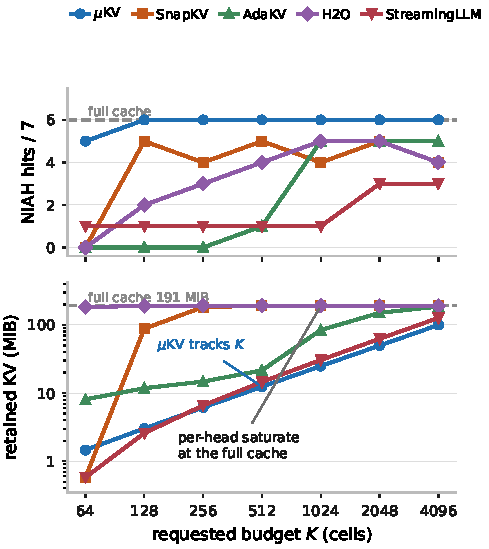
\includegraphics[width=0.92\columnwidth]{figures/fig_ksweep.pdf}
\caption{Requested budget vs.\ delivered cache and retrieval, 8K context (Llama-3.2-1B).}
\label{fig:ksweep}
\end{figure}

\subsection{How small can the budget go?}
\label{sec:eval-ksweep}
Every prior eviction paper plots quality against the budget $K$; we plot both what each policy \emph{delivers} for that budget and what it retrieves (Fig.~\ref{fig:ksweep}, 8K context, 7 depths per point).

The lower panel is the realizability gap measured rather than argued. $\mu$KV's retained cache doubles with $K$ exactly as requested, 1.5 to 99.8\,MiB across a 64$\times$ sweep. No per-head policy does. SnapKV saturates at the full cache by $K{=}256$: ask it for a 512-cell budget and it holds 190.5 of 190.7\,MiB, the entire prompt. H2O is pinned at the full cache from $K{=}64$. Ada-KV climbs toward the full cache instead of tracking the budget, reaching 150\,MiB at $K{=}2048$. Their nominal budgets are not what the engine stores, because a per-head keep-set is a union over heads that a sequence-level cache cannot compact below.

The upper panel shows what that buys. At $K{=}1024$, $\mu$KV matches the full cache at 6/7 on 24.9\,MiB, while SnapKV reaches 4/7 on 190.7\,MiB and Ada-KV 5/7 on 84.0\,MiB --- the best accuracy on $7.7\times$ less memory than the nearest competitor. $\mu$KV holds full-cache accuracy down to $K{=}128$ (3.0\,MiB, a 64$\times$ reduction) and breaks only at $K{=}64$, where it drops to 5/7. StreamingLLM behaves as designed and fails: it compacts well but a sliding window always evicts the middle of the prompt, where the needle sits, so it retrieves 1/7 at almost every budget. Two results deserve stating plainly against our own interest: Ada-KV, the closest prior art, returns 0/7 at $K\le256$ on this workload, and $\mu$KV's own knee at $K{=}64$ is a real quality loss, not a benchmark artifact.

\subsection{Cache size is not a temperature actuator}
\label{sec:eval-tdak}

We also tested coupling the cache budget itself to DDR temperature (a four-tier ladder over $K\in\{256,512,768,1024\}$, symmetric and ratcheted variants, under cool and co-loaded regimes). The mechanism works, but the result is negative and we do not ship it: cache size controls throughput, wall time, and energy, not peak temperature. Halving $K$ under co-load left peak DDR unchanged because the co-load dominates the thermal budget, and on a cool phone a smaller cache runs hotter at peak because the saved bandwidth converts to speed and power. Frequency remains the only lever that caps heat, which is why the shipped design pairs eviction (efficiency) with the clock watchdog (temperature) and nothing else.

\subsection{Watchdog: gradual clock reduction before the kernel throttle}
\label{sec:eval-thermal}

Figure~\ref{fig:bonsai-thermal} traces three runs. The watchdog belongs to $\mu$KV and is never given to a baseline in any comparison; the \texttt{vanilla+watchdog} trace is an \emph{ablation} only, included because $\mu$KV finishes before reaching the cliff and so cannot show the clock lever in isolation. Dotted lines mark the 883\,MHz throttle floor and the 50\,\textdegree C battery and skin thresholds. The watchdog's target is \emph{sustained, throttle-free operation}: keeping a long-running workload just below the temperature at which the vendor deep-throttles, so the phone sustains work at a stable equilibrium instead of hitting a cliff. It is a userspace daemon sampling battery, skin, DDR and CPU at 2\,Hz that lowers the big-core cap one step at a time, never raising it, and runs only under $\mu$KV. We anchor the ladder to the \emph{measured} trigger: on this SoC the vendor deep-throttle fires the instant battery reaches 50\,\textdegree C.

The orange trace of Figure~\ref{fig:bonsai-thermal} demonstrates this on the workload that actually reaches the cliff. Without the watchdog, vanilla Bonsai-8B climbs to a 50.2\,\textdegree C battery and deep-throttles to 883\,MHz for 125\,s. With it, the ladder engages at 46--49\,\textdegree C and steps the cap 1497/1382/1267/1132\,MHz as heat rises; battery peaks at 49.0\,\textdegree C and the 50\,\textdegree C trigger is never reached, so the deep throttle collapses from 125\,s to 1\,s. The watchdog buys \emph{thermal sustainability}, not throughput: it is complementary to the cache lever, which owns speed and energy. In the cold-start runs of Table~\ref{tab:master-wikitext} $\mu$KV finishes fast enough not to need it at all.

Two clarifications. First, the mild vendor step from 1632 to 1498\,MHz near 40\,\textdegree C skin is ordinary DVFS, not throttling; we reserve the term for the deep drop toward 883\,MHz. Second, because this decode is bandwidth-bound the clock is not the throughput limiter, so preventing the throttle adds no speed---vanilla runs at 1.0\,tps and 86\,minutes with or without the watchdog. The watchdog therefore buys \emph{thermal sustainability}, not throughput: it is complementary to $\mu$KV, which owns speed and efficiency through cache compaction. In the cold-start systems runs of Table~\ref{tab:master-wikitext}, $\mu$KV finishes fast enough that no policy reaches a deep throttle at all, so its advantage there is efficiency (2.6$\times$ less time, 5.4\,\textdegree C cooler DDR); the watchdog is the insurance for the sustained-hot regime, where a workload would otherwise cross 50\,\textdegree C, and the orange trace of Fig.~\ref{fig:bonsai-thermal} shows it holding exactly that line.



\subsection{Energy-aware scheduling by battery state}
\label{sec:eval-energy}

The watchdog holds temperature; a second controller holds energy. Per request, from the battery
state the phone reports, it picks the GPU clock cap, the cache budget and the output cap from a
measured cost table, walking down a ladder of plans only while a step saves more energy than it
costs in time at the tier's exchange rate (1.5, 0.8, 0.5 for the healthy, mid and low tiers) and
stays inside a time budget. The controls were measured first. The GPU cap trades prefill energy
for prefill time (1200 to 902\,MHz: 1428 to 1154\,J for 221 to 263\,s on a 4096-token request);
decode is bandwidth-bound and barely feels it, so prefill at 1200 with decode capped at 902 saves
6 percent for 1.5 percent of time and is the best point by energy-delay product, the
two-configuration schedule of Kim, Imes and Hoffmann~\cite{kim2015racepace}. The CPU clock is not
an energy lever (flat within 7 percent from 883 to 1632\,MHz) and stays with the watchdog. A GPU cap ladder at DDR 60, 62 and 63.5\,$^\circ$C, stepping before the vendor's trip, gives 7 percent less energy and a 15\,$^\circ$C lower DDR peak at equal time on the 4096-token request (n=3). The
cache is the CPU lever only against the full cache; below $K{=}1024$ the tiers save 3 to 4 percent
for a 37 to 42 percent quality loss, so $K$ stays at 1024. Output length is linear at 0.17 to
0.21\,J per token, which makes the cap the largest lever when the caller left the length open.

\begin{figure}[t]
\centering
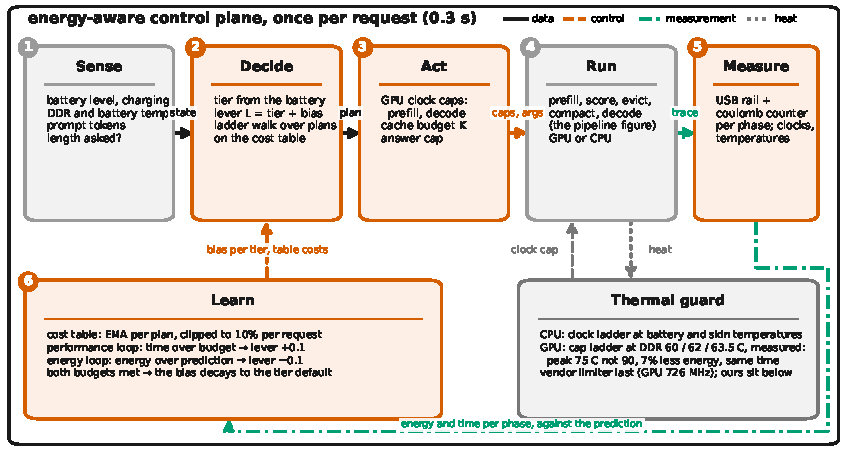
\includegraphics[width=\linewidth]{fig_control_plane.pdf}
\caption{The energy-aware control plane: sense, decide, act, run, measure, learn, once per request,
with the thermal guard beside it. Solid: data. Dashed: control. Dash-dot: measurement. Dotted: heat.}
\label{fig:controlplane}
\end{figure}

Two loops act on model error in the JouleGuard manner~\cite{hoffmann2015jouleguard}: a time
overrun nudges a lever toward performance, an energy overrun toward energy, and the bias decays
when both budgets are met. Provoked with four spinning cores and with an external 726\,MHz cap,
each loop fired only on the disturbance meant for it, and the phone's own limiter, which trips at
DDR 64\,\textdegree C, was handled the same way. A decision costs 0.3\,s.

\begin{table}[t]
\centering\small
\caption{What the scheduler does at each battery tier and what it costs: cooled cells on the cable,
and the real discharge on the battery. Llama-3.2-1B, 9737-token prompt, OnePlus 15.}
\label{tab:energy-aware}
\begin{tabular}{@{}lllrrr@{}}
\toprule
\textbf{battery} & \textbf{GPU plan} & \textbf{cap} & \textbf{cable, J} & \textbf{battery, J} & \textbf{battery, s} \\
\midrule
mains or above 50\% & 1200, decode 902 & 4096 & 1336 (1428 uncapped) & 885 & 280 \\
21 to 50\%          & 1200, decode 726 & 1024 & 577 (at 902)          & 748 & 210 \\
20\% or below       & 902              & 512  & 500                   & 506 & 177 \\
GPU unavailable     & CPU, $K{=}1024$  & by tier & 822 (1024 tokens)  & --  & --  \\
\bottomrule
\end{tabular}
\end{table}

\begin{figure}[t]
\centering

\includegraphics[width=\linewidth]{fig_discharge_timeline.pdf}
\caption{The scheduler on a real discharge: energy and time per request against the battery level
it read, with tier bands, the plan chosen and the cap. Hatched: USB cable in.}
\label{fig:discharge}
\end{figure}

A loop resident on the phone then ran 123 requests from 91 to 11 percent with charging disabled
and no forced state (Figure~\ref{fig:discharge}, Table~\ref{tab:energy-aware}). The scheduler
switched on the first request past each threshold, and the tiers cost 885, 748 and 506\,J per
request: 15 and 43 percent less than the healthy tier, with time down 25 and 37 percent. On the
battery the phone is a different machine from the phone on the cable: the OEM runs the GPU cooler
when unplugged and caps prefill at 726\,MHz within a minute, so the same healthy request costs
885\,J instead of 1274, and there the answer and prefill caps carry the saving while the
decode-clock lever is pre-empted by the vendor. The cost table re-learned that regime in three
requests. No shipped phone changes an LLM's clock, context or answer length by battery state, and
the closest research system excludes battery level by design~\cite{zou2026enerinfer}; the per-rail
PowerBench measurements on this phone~\cite{cai2026powerbench} and the FUSE governor
study~\cite{zhang2025fusellm} agree with our per-token costs.

\subsection{Cross-model replication}
The headline Phi-3 result replicates on Llama-3.2-1B and gemma-2-2b-it. On Llama-1B at 16K decode $\mu$KV reaches \good{16.29\,tps} (vanilla 4.87, AdaKV 5.90) at \good{446\,mWh} (vanilla 634, AdaKV 653); on gemma-2-2b, \good{7.17\,tps} (vanilla 3.35, AdaKV 2.69) at \good{847\,mWh} (vanilla 1322, AdaKV 1367). $\mu$KV is the fastest and lowest-energy policy on every model, holds DDR 8--10\,\textdegree C below the cliff that vanilla and AdaKV approach, and uses the least RSS.
\label{sec:eval-cross}

The headline Phi-3 result replicates on Llama-3.2-1B and gemma-2-2b-it (Table~\ref{tab:master-wikitext}, bottom 6 rows). On Llama-1B at 16K decode, $\mu$KV reaches \good{16.29\,tps} (vs vanilla 4.87, AdaKV 5.90) at \good{446\,mWh} system energy (vs vanilla 634, AdaKV 653). On gemma-2-2b, \good{7.17\,tps} (vs vanilla 3.35, AdaKV 2.69) at \good{847\,mWh} (vs 1322, 1367). The pattern is consistent: $\mu$KV is the fastest and the lowest-energy policy on every model, holds DDR 8--10\,\textdegree C below the cliff vanilla and AdaKV approach, and uses the least RSS. PPL on Llama-1B and Gemma-2B shows the count-$\alpha$ saturation effect (Sec.~\ref{sec:design}, the dispatcher v1) over-allocating anchors for smaller models; the mass-$\alpha$ dispatcher rebalances toward recent on these regimes, closing the quality gap in follow-on sweeps.

\subsection{Vision-language models}
\label{sec:vlm}
Image tokens enter the same KV cache as text tokens, so $\mu$KV applies to a vision-language model unchanged. On Qwen2.5-VL-3B with one image and a 1024-token answer it cut the live cache from 144 to 23\,MiB, a 6.3$\times$ reduction, with prefill and decode within 1\% of the full cache and answers still correct. One engine change was needed: multimodal position encoding gives every token of an image the same position index (4105 cells shared 110 positions in our run), and llama.cpp removes cells by position range, so it cannot express a per-token keep mask on such a cache. We added a cell-index removal call used only when the cache is multimodal; the text path is untouched and still bit-identical. At this size the cache is small next to the weights, so the win is memory, not speed; multi-image and video inputs, where the cache grows into gigabytes, are where throughput should follow.

\subsection{Limitations and scope}
\label{sec:limitations}

\emph{Device.} All measurements on a single OnePlus 15 (Snapdragon 8 Elite Gen 5). Watchdog thresholds are device-specific; the calibration protocol (10 measured pre-throttle events on the vanilla baseline) generalizes but the specific tier values do not.
\emph{Energy.} System energy via USB rail $V\cdot I$ integration with charging disabled throughout each cell. This is total-device energy (CPU, DDR, modem, screen-off); we cannot isolate DDR-specific energy without a die-attached power meter.


\paragraph{Why CPU-only.} Sustained decode on the mobile GPU is bandwidth-saturated, so eviction has little throughput headroom to recover there; the CPU is where a bounded cache converts directly into speed and energy. The GPU results (\S\ref{sec:gpu-results}) show the thermal and energy story still holds, and the realizability finding is engine-level, not processor-level.
\section{Conclusion}
\label{sec:conclusion}

$\mu$KV is a mobile inference pipeline that makes attention-driven KV eviction viable on a phone and measures it end-to-end on a OnePlus 15: a cheap $O(H)$ per-head budget signal, in-graph scoring with sequence-level compaction that keeps the evictor on the fast path, and a reduce-only frequency watchdog. We report what it does not do as plainly as what it does: no configuration of the cache actuator caps peak temperature under external co-load, so frequency remains the only thermal lever; and aggressive eviction costs verbatim recall of dropped spans even as it preserves prediction and retrieval. The useful takeaway is the substrate, not the trophy: on-device LLM serving should close the loop between attention-driven cache state and hardware sensors per request --- the cache is the phone's \emph{efficiency} actuator, the clock its \emph{temperature} actuator, and the two compose.


\paragraph{Reproducibility.} We release the \texttt{eviction\ub bench} binary with all six policy implementations, the multi-sensor watchdog daemon, the energy fallback chain, and the host-side harnesses for Wave-11 chunk-pair PPL, NIAH Tier-1, and LongBench at \url{[anonymized URL]}. Phone-side scripts target Android NDK aarch64; host-side LongBench builds against \texttt{llama.cpp} with CUDA. All measurements use seed 42 throughout; the protocol scripts pin DVFS to the performance governor and the kernel cap (1632\,MHz on Snapdragon 8 Elite Gen 5) before each cell. All raw \texttt{meta.\allowbreak json} and \texttt{stress.\allowbreak csv} artifacts referenced in the tables are included in the release.

\begin{thebibliography}{99}
\small
\bibitem{zhang2023h2o} Z. Zhang et al. ``H2O: Heavy-Hitter Oracle for Efficient Generative Inference of LLMs.'' NeurIPS, 2023.
\bibitem{xiao2024streamingllm} G. Xiao et al. ``Efficient Streaming Language Models with Attention Sinks.'' ICLR, 2024.
\bibitem{oren2024tova} M. Oren et al. ``Transformers are Multi-State RNNs.'' arXiv:2401.06104, 2024.
\bibitem{li2024snapkv} Y. Li et al. ``SnapKV: LLM Knows What You're Looking For Before Generation.'' NeurIPS, 2024.
\bibitem{liu2024kivi} Z. Liu et al. ``KIVI: Tuning-Free Asymmetric 2bit Quantization for KV Cache.'' arXiv:2402.02750, 2024.
\bibitem{feng2025adakv} Y. Feng et al. ``Ada-KV: Optimizing KV Cache Eviction by Adaptive Budget Allocation.'' NeurIPS, 2025.
\bibitem{feng2025criticalkv} Y. Feng et al. ``CriticalKV: A Perturbation Perspective on KV Cache Eviction.'' ICML, 2026.
\bibitem{feng2025defensivekv} Y. Feng et al. ``DefensiveKV: Worst-Case Risk Control for KV Cache Eviction.'' ICLR, 2026.
\bibitem{gu2025ahakv} Y. Gu et al. ``AhaKV: Adaptive Holistic Attention-Driven KV Cache Eviction.'' arXiv:2506.03762, 2025.
\bibitem{hsieh2024ruler} C.-P. Hsieh et al. ``RULER: What's the Real Context Size of Your Long-Context Models?'' arXiv:2404.06654, 2024.
\bibitem{bai2023longbench} Y. Bai et al. ``LongBench: A Bilingual, Multitask Benchmark for Long Context Understanding.'' arXiv:2308.14508, 2023.
\bibitem{dao2022flashattention} T. Dao et al. ``FlashAttention: Fast and Memory-Efficient Exact Attention.'' NeurIPS, 2022.
\bibitem{dao2023flashattention2} T. Dao. ``FlashAttention-2: Faster Attention with Better Parallelism.'' arXiv:2307.08691, 2023.
\bibitem{song2024powerinfer2} Y. Song et al. ``PowerInfer-2: Fast LLM Inference on a Smartphone.'' arXiv:2406.06282, 2024.
\bibitem{alizadeh2023llm} K. Alizadeh et al. ``LLM in a Flash: Efficient Inference with Limited Memory.'' arXiv:2312.11514, 2023.
\bibitem{llamacpp} G. Gerganov. ``llama.cpp.'' \url{https://github.com/ggerganov/llama.cpp}.
\bibitem{qualcommbcl} Qualcomm. ``Battery Current Limit (BCL) for Snapdragon Platforms.'' Whitepaper, 2023.
\bibitem{michel2019sixteen} P. Michel et al. ``Are Sixteen Heads Really Better than One?'' NeurIPS, 2019.
\bibitem{voita2019analyzing} E. Voita et al. ``Analyzing Multi-Head Self-Attention.'' ACL, 2019.
\bibitem{kim2025kvzip} J.-H. Kim et al. ``KVzip: Query-Agnostic KV Cache Compression with Context Reconstruction.'' NeurIPS, 2025.
\bibitem{liu2025percache} K. Liu, L. Zeng, L. Xu, B. Yang, Z. Yan. ``PerCache: Predictive Hierarchical Cache for RAG Applications on Mobile Devices.'' arXiv:2601.11553, 2025.
\bibitem{mlcllm} MLC Team. ``MLC-LLM: Universal LLM Deployment.'' \url{https://github.com/mlc-ai/mlc-llm}.
\bibitem{kim2021ztt} S. Kim et al. ``zTT: Learning-Based DVFS with Zero Thermal Throttling for Mobile Devices.'' MobiSys, 2021.
\bibitem{liu2022fuse} S. Liu et al. ``FUSE: Fine-Grained Power Management for Mobile Devices.'' SenSys, 2022.
\bibitem{cai2025rkv} X. Cai et al. ``R-KV: Redundancy-aware KV Cache Compression for Reasoning Models.'' arXiv:2505.24133, 2025.
\bibitem{zhou2024dynamickv} X. Zhou et al. ``DynamicKV: Task-Aware Adaptive KV Cache Compression for Long Context LLMs.'' arXiv:2412.14838, 2024.
\bibitem{prismml2026bonsai} PrismML. ``Bonsai: Commercially Viable 1-bit LLMs.'' 2026. \url{https://prismml.com/news/bonsai-8b}.
\bibitem{hoffmann2015jouleguard} H. Hoffmann. ``JouleGuard: Energy Guarantees for Approximate Applications.'' SOSP, 2015.
\bibitem{kim2015racepace} D. H. K. Kim, C. Imes, and H. Hoffmann. ``Racing and Pacing to Idle: Theoretical and Empirical Analysis of Energy Optimization Heuristics.'' CPSNA, 2015.
\bibitem{zou2026enerinfer} B. Zou et al. ``EnerInfer: Energy-Aware On-Device LLM Inference.'' arXiv:2606.23001, 2026.
\bibitem{cai2026powerbench} G. Cai et al. ``Is Your NPU Ready for LLMs? A Power Benchmark of On-Device Inference.'' arXiv:2607.05475, 2026.
\bibitem{zhang2025fusellm} Z. Zhang et al. ``Dissecting the Impact of Mobile DVFS Governors on LLM Inference Performance and Energy Efficiency.'' arXiv:2507.02135, 2025.
\end{thebibliography}

\end{document}
